%%% template.annotated.tex
%%%
%%% This LaTeX source document can be used as the basis for your technical
%%% paper or abstract. Unlike ``template.tex,'' this version of the source
%%% document contains documentation of each of the commands and definitions
%%% that should be used in the preparation of your formatted document.
%%% 
%%% The parameter given to the ``acmsiggraph'' LaTeX class in the 
%%% ``\documentclass'' command controls several features of the formatted 
%%% output: the presence or absence of hyperlinked icons just prior to the 
%%% first section of the paper, the amount of space left clear for the ACM
%%% copyright notice, the presence or absence of line numbers and submission
%%% ID, and the presence or absence of an appropriate ``preprint'' notice.
%%% 
%%% If you are preparing a paper for presentation in the Technical Papers
%%% program at one of our two annual flagship conferences, held in North 
%%% America (SIGGRAPH) or Asia (SIGGRAPH Asia), you should use ``annual''
%%% as the parameter.
%%%
%%% If you are preparing a paper for presentation at one of our sponsored
%%% events, including SIGGRAPH and SIGGRAPH Asia, but not in those events' 
%%% Technical Papers program, you should use ``sponsored'' as the parameter.
%%% (Technical Briefs and Game Papers presented at our annual flagship 
%%% events fall into this category, as do papers accepted to other SIGGRAPH-
%%% sponsored events, such as I3D or ETRA or VRCAI.)
%%%
%%% If you are preparing a version of your content for review, you should
%%% use ``review'' as the parameter. Line numbers will be added to your 
%%% paper, and the submission ID value will be printed across the top of 
%%% each page of your paper. (Use the submission ID as the parameter to the
%%% ``TOGonlineID'' command, below.)
%%%
%%% If you are preparing an abstract, typically one to four pages in 
%%% length, you should use ``abstract'' as the parameter. No space will 
%%% be left clear for the ACM copyright notice, as copyright is not 
%%% transferred for abstracts. A small permission notice will be added
%%% to your content during production in the footer of the first page.
%%%
%%% If you are preparing a preprint of your content, you should use
%%% ``preprint'' as the parameter. This is primarily for annual conference
%%% papers; a header reading ``To appear in ACM TOG X(Y)'' will appear on
%%% each page of the formatted output (where X is the volume and Y is the 
%%% number of the issue in which it will be published).

\documentclass[annual]{acmsiggraph}

%%% Definitions and commands that begin with ``\TOG'' are meant to be used
%%% in the preparation of papers to be presented in the Technical Papers
%%% program at one of our annual flagship events - SIGGRAPH and SIGGRAPH 
%%% Asia. You can safely ignore these definitions and commands if your 
%%% content is to be presented in some other venue.

%%% ``\TOGonlineid'' should be filled with the online ID value you received
%%% when you submitted your technical paper. It will be printed out if you 
%%% prepare a ``review'' version of your paper.

\TOGonlineid{45678}

%%% Should your technical paper be accepted, you will be given three pieces
%%% of information: the volume and number of the issue of the ACM Transactions
%%% on Graphics journal in which your paper will be published, and the 
%%% ``article DOI'' value, which is unique to your paper and provides the 
%%% link to your paper's page in the ACM Digital Library. Fill in the 
%%% ``\TOGvolume,'' ``\TOGnumber,'' and ``\TOGarticleDOI'' definitions with
%%% the three pieces of information you receive.

\TOGvolume{0}
\TOGnumber{0}
\TOGarticleDOI{1111111.2222222}

%%% By default, your technical paper will contain hyperlinked icons which 
%%% point to your paper's article page in the ACM Digital Library, and to 
%%% the paper itself in the ACM Digital Library. You may wish to add one 
%%% or more links to your own resources. If any of the following four 
%%% definitions have URLs in them, an appropriate hyperlinked icon will be
%%% added to the list. 

\TOGprojectURL{}
\TOGvideoURL{}
\TOGdataURL{}
\TOGcodeURL{}

%%% Define the title of your paper here. Use capital letters as appropriate.
%%% Setting the entire title in upper-case letters is not correct, nor is 
%%% capitalizing only the first letter of the title.

\title{Designing Rhythm Game Interfaces for Touchscreen Devices}

%%% Define the author list in the ``\author'' command. The ``\thanks'' 
%%% field can be used to define an e-mail address for the author.
%%% The ``\pdfauthor'' field should contain a comma-separated list of the
%%% authors of the paper, and is used, along with the title and keyword
%%% data, for PDF metadata. (To see this metadata, open the PDF in Adobe 
%%% Reader and select ``File > Properties > Description.''

\author{Philip H. Peng and Stephen H. Lane\thanks{e-mail:pengp@stwing.upenn.edu, shlane@cis.upenn.edu}\\University of Pennsylvania at Philadelphia, PA}
\pdfauthor{Philip H. Peng}

%%% User-defined keywords.

\keywords{rhythm game, touchscreen, user interface, prototype}

%%% End of the document preamble, start of the document.

\begin{document}

%%% A ``teaser'' image appears below the title and affiliation and above
%%% the two-column body of the paper. This is optional, but if you wish
%%% to include such an image, the commented-out code, below, can be used
%%% as an example. Please note that the inclusion of a ``teaser'' image
%%% may move the copyright space to the bottom of the right-hand column
%%% on the first page of your formatted output. This is acceptable.

%
% \teaser{
%   \includegraphics[width=1\linewidth]{figure_teaser}
%   \caption{Left: Eight different user interface designs were prototyped in this study, shown in the ''Mode Select'' screen of the app. Center: Gameplay %featuring Design \#1: Falling Notes. Right: Gameplay featuring Design \#4: Grid.}
 %}

%%% The ``\maketitle'' command uses the author and title information 
%%% defined above, and prepares the formatted title.

\maketitle

%%% The first section of your paper. 

\section{Introduction}
\vspace{-6pt}
Over the past few years, touchscreen devices have become increasingly common in the consumer market. With the adoption of this new input paradigm comes the natural expectation of increased software support for new touch-focused interfaces, allowing for faster and more natural human-device interactions~\cite{hayes_thesis}.

One area that touchscreen support can be leveraged is in the design of rhythm games. Rhythm games often focus the player's beat recognition abilities, which can be measured by the tapping of objects on a touchscreen to the rhythm of the song. The success of a rhythm game depends on two main factors: 1) user responsiveness during gameplay, and 2) gameplay experience as a whole.

In this study, different touchscreen user interface designs were compared for user responsiveness and gameplay experience through the development, release, and data/user feedback collection of \textit{Beats2 Prototypes}, a rhythm game designed for Android tablets.

%%% The ``CRCatlist'' environment defines one or more ACM ``Computing Review''
%%% (or ``CR'') categories, used for indexing your work. For more information
%%% on CR categories, please see http://www.acm.org/class/1998.
%\vspace{-6pt}
%\begin{CRcatlist}
%  \CRcat{H.5.2}{Information Interfaces and Presentation}{User Interfaces}{Graphical user interfaces (GUI)}
%  \CRcat{H.5.2}{Information Interfaces and Presentation}{User Interfaces}{Prototyping};
%\end{CRcatlist}

%%% The ``\keywordlist'' prints out the user-defined keywords.
%\vspace{-12pt}
%\keywordlist

\section{Our Approach}
\vspace{-6pt}
This study compared rhythm game interfaces through the following three stages: \textit{Design}, \textit{Prototype}, and \textit{Evaluation}.

In the \textit{Design} stage, a wide range of existing commercial rhythm games were analyzed and categorized based on their interface characteristics. These categories were used to draft eight simplified interface designs, as shown in Figure~\ref{fig:demo_interfaces}.

\begin{figure}[htb!]
	\begin{center}
		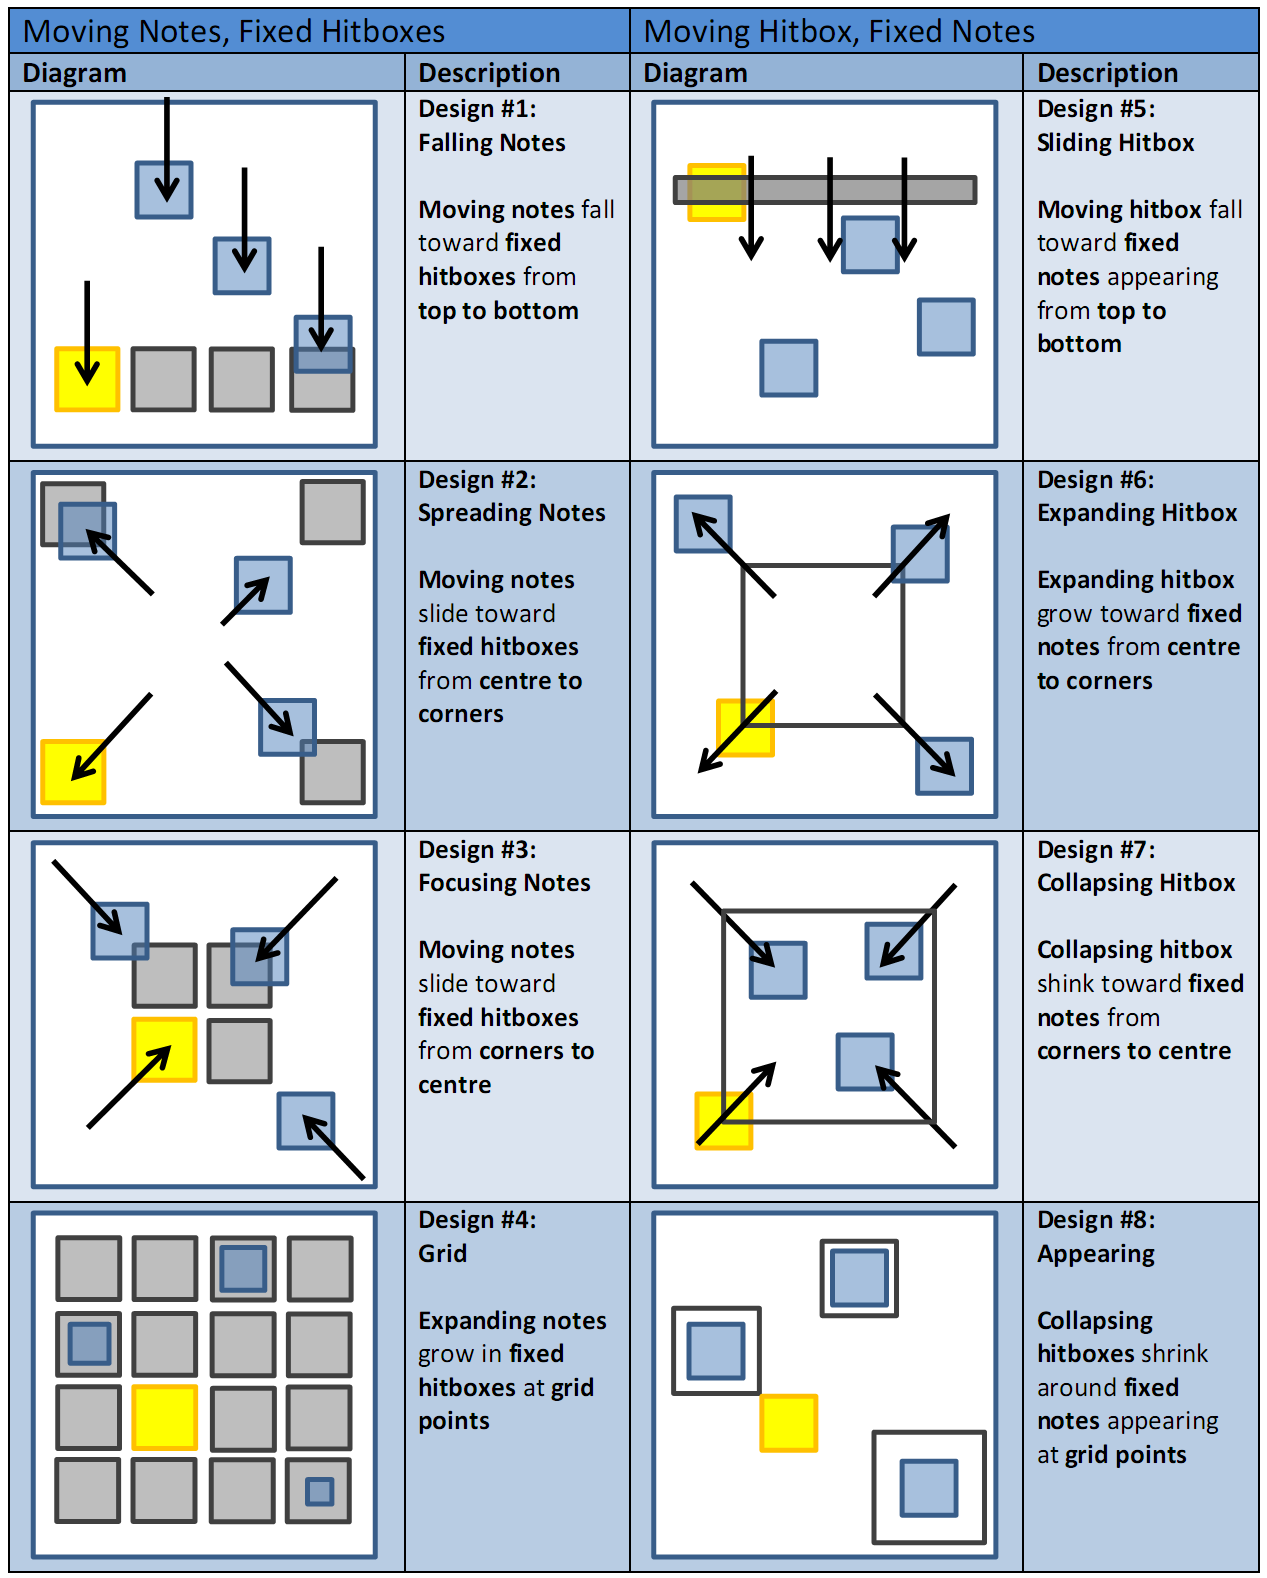
\includegraphics[width=0.95\linewidth]{figure_demo_interfaces}
	\end{center}
	\vspace{-6pt}
	\caption{Interfaces designs studied in the prototype app.}
	\label{fig:demo_interfaces}
\end{figure}

In the \textit{Prototyping} stage of the study, a prototype rhythm game was created implementing the designs drafted in the previous \textit{Design} stage as eight selectable ''Modes''. The game was titled \textit{Beats2 Prototypes} and developed using the \textit{Unity3} game engine, targeting Android tablets. In the starting mode select screen, the player would choose one of the eight game modes to play. In the following gameplay screen, the player would play through the rhythm game featuring the interface design selected but with the same song data, note patterns, and scoring system. At the end of the song, a feedback form would display, prompting the player to give 1-5 star ratings on various aspects of the gameplay.

In the \textit{Evaluation} stage of the study, the rhythm game prototype was published on \textit{Google Play}, an Android app store from Google. Through the use of a built-in tracker, data was collected from app users for comparing each individual interface designs. The score and timing accuracy of note hits were used as quantitative metrics for comparing user responsiveness. The feedback ratings, given on the five categories: \textit{Challenge, Intuitive, Fun, Unique,} and \textit{Overall} (losely based on the \textit{GameFlow} model~\cite{gameflow}), were used as qualitative metrics for comparing gameplay experience. The results of these comparisons are shown in Figure~\ref{fig:chart_results}.

\begin{figure}[htb!]
	\begin{center}
		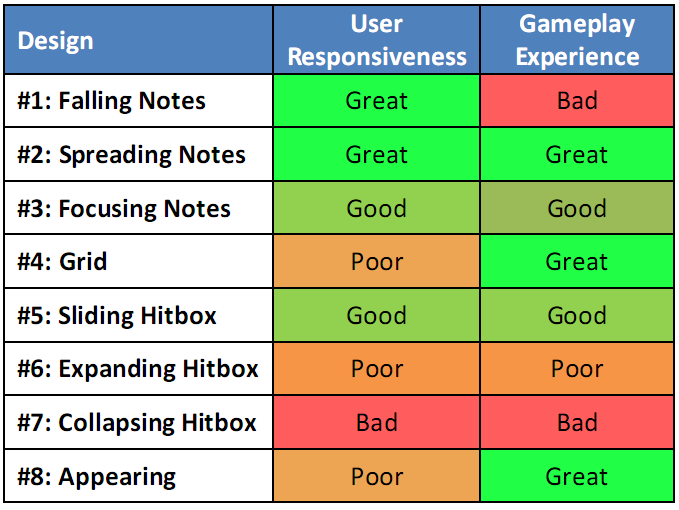
\includegraphics[width=0.95\linewidth]{figure_chart_results}
	\end{center}
	\vspace{-6pt}
	\caption{Relative comparisons of the studied interface designs.}
	\label{fig:chart_results}
\end{figure}

Of the eight designs studied, Design \#2 is the best candidate for usage in future rhythm game development on touchscreen devices. These results can also be applied in the design of user interfaces for other future touch-based applications. As touchscreen technology become more and more commonplace, user interfaces for interacting with touchscreen elements in time-critical scenarios (such as military or medical applications) will benefit from designs improving user responsiveness as well as user experience.

\bibliographystyle{acmsiggraph}
\bibliography{template}
\end{document}
